\scanpage{23}
\deleted{Dans le cas général (motifs pas nécessairement constants) la connaissance des opérations $\Theta_X$ sur les $V_{\mathbb{C}}$ $(V\in\operatorname{Ob}\mathcal{M})$ implique-t-elle celle des éléments des structures $1^{\mathrm o}$ et $2^{\mathrm o}$, \deleted{ou dans quelle mesure du moins?}}
\margin{\deleted{\uuline{oui}} ??}

\margin{\begin{tikzpicture}
\node[inner sep=1pt,align=left,text width=.93\marginparwidth] (rubrique) {Situation abstraite de la donnée d'une connexion intégrable un foncteur fibre.};
\draw (rubrique.north west) -- (rubrique.south west) -- (rubrique.south east);
\end{tikzpicture}}

\begin{center}\rule[.2ex]{2cm}{.4pt}\end{center}

Considérons une $\otimes$-catégorie $\mathcal{M}$ sur corps $k_0$, soit $K$ une extension de $k_0$. On suppose donné un foncteur fibre à valeurs en $k_0$, \unsure{donc|dans} $\mathcal{M}$. avec ce foncteur fibre est donné par $G$ sur $k_0$, $\mathcal{M}$ s'identifie avec \unsure{``$G$-$k_0$-modules\ldots|$G$-$k_0$-modules\ldots} On veut déterminer les façons de mettre, sur chaque $V\otimes_{k_0}K$ une connexion intégrable \inserted{rel : $K/k_0$}, \uline{fonctorielle} en $V$, \inserted{et ``compatible avec $\otimes$''.}

Or il y en a déjà une $\unsure{\Theta_0|\text{\textcircled{H}}_0}$, déduit des $k$-structures dont on \deleted{\unsure{suppose}} dispose déjà sur chaque $V\otimes_{k_0}K$. Une autre connexion \deleted{\unsure{intégrable}} \inserted{sur $V$} sera donc de la forme
\[
 \Theta_X^V={\Theta_0}_X^V+\omega^V(X)^{\deleted{\unsure{V|x}}}
\]
\unsure{où|ou}
\[
 \omega^V\deleted{\unsure{(X)|\in}}:\operatorname{Dér}_{k_0}(K/k_0)\longrightarrow
 \operatorname{End}_K(V_K\unsure{)}\,\text{est \uline{$K$-linéaire}}
\]
\[
 \Theta_X^V(\varphi)={\Theta_0}_X^V(\varphi)+\omega^V(X)(\varphi)
\]
Si on veut choisir les $\Theta_X^V$ pour tt $V$, de façon compatible avec multiplication, on trouve que \deleted{$\unsure{\omega^V|\omega}\unsure{\Theta_X|(X)}$} $\omega^V(X)$, pour $V$ variable, est une ``dérivation'' du foncteur fibre \deleted{\unsure{donné}}\inserted{$F_K$}, donc défini par un élément de \deleted{Lie} $\mathfrak{g}_K$, où $\mathfrak{g}=\operatorname{Lie}G$. Soit $\omega(X)\in\mathfrak{g}_K$ cet élément.
% archive sheet number: 22
